% = = = = = = = = = = = = = = = = = = = = = %
%               Discussion                  %
% = = = = = = = = = = = = = = = = = = = = = %

\let\clearpage\relax

\chapter{Discussion \& Future Work} %syq

\section{Load-Store Unit}
\subsection{Problem}
The most significant characteristic of an out-of-order core is that the order of executed instructions is random, including memory access instructions. With the help of ROB, we can ensure that the results of all the integer and floating point instructions are correct. However, without specifically designed load-store unit, we cannot ensure that the content in the memory is consistent. For example, consider the following two instructions.
\begin{equation*}
    \centering
    \texttt{sw x1, 0(x2); lw x3, 0(x4)}
\end{equation*}
If the addresses stored in \texttt{x2} and \texttt{x4} are identical, there exists potential memory data dependency, i.e., memory alias, under which circumstance the two instructions must be executed sequentially. Thus, we need a load-store unit to ensure that the memory consistency is kept. As mentioned in the issue logic for memory access instructions, currently our strategy is to consider all store instructions as barriers, i.e., we don't care the order of load instructions between two store instructions, but the store instructions must be executed sequentially.

However, we still need to consider the case of branch mis-prediction. If a branch mis-prediction occurs, speculative load instructions will not influence the memory consistency, but speculative store instructions will. For example, a store instruction following a branch mis-prediction will write the wrong value to the memory, which is irrevocable.

\subsection{Current Solution \& Future Work}
To resolve this conflict, a load-store unit is necessary to keep memory consistency. Currently we design a simple store buffer simulated in Verilator. As it is implemented in software, there is no limitation in terms of size and delay. When speculative store instructions are executed in the execution stage, the processor will send a store request to the store buffer. Only when these store instructions commit, the store buffer will write the data to corresponding memory addresses. If a branch mis-prediction occurs and sends a recover signal, the content of store buffer will be immediately flushed. Furthermore, when load instructions are executed, we will first check whether there exists store instructions that share the same address with load instructions. If so, we directly return the data from store buffer. Otherwise, we load the data from main memory as usual. Fig.~\ref{fig:store-buffer} shows a simplified diagram of store buffer in our memory access system.

\begin{figure}[!htp]
    \centering
    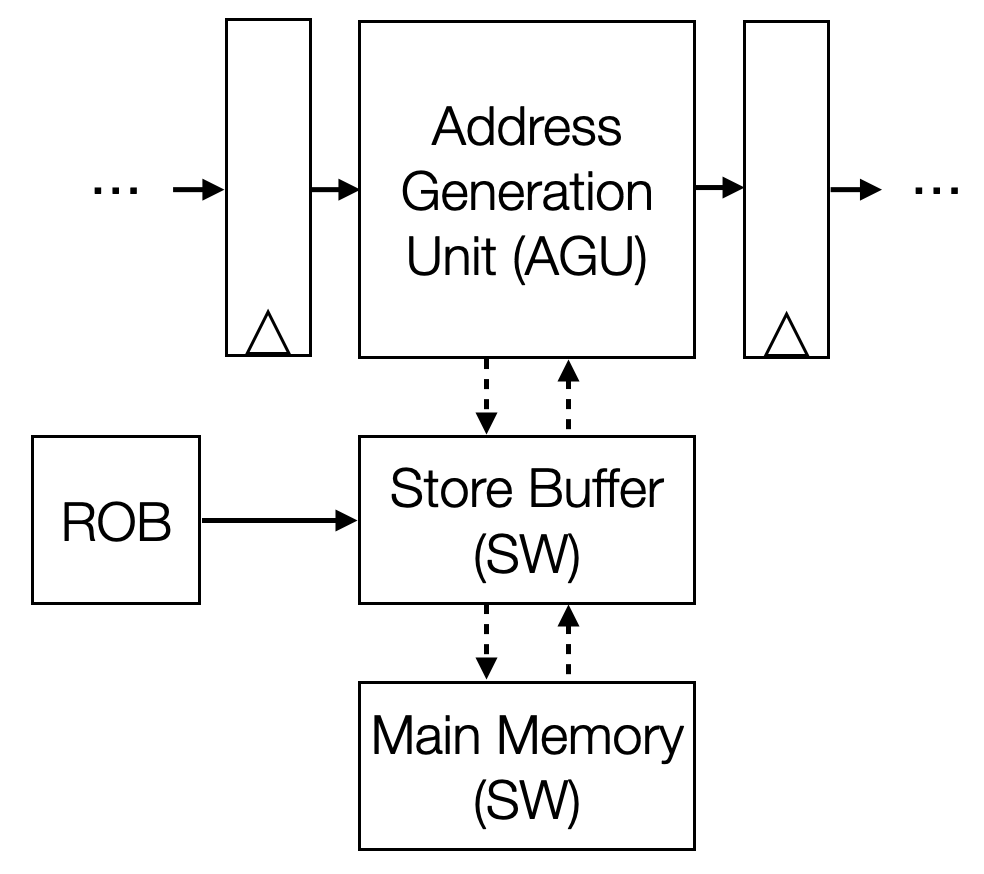
\includegraphics[width=0.4\textwidth]{figure/store_buffer.png}
    \caption{Current solution of store buffer.}
    \label{fig:store-buffer}
\end{figure}

In the future, we may implement the store buffer in RTL design. We may also further improve the performance of memory access by introducing more complicated load-store unit, e.g., miss status handling register (MSHR).


\section{Pipeline Optimization}
\subsection{Problem}

We designed our Out-of-order ten-stage processor based on several designs such as the "BOOM" design mentioned in section \ref{section: BOOM}. However, there are still some room for optimizations in mircoarchitectures. Two stages that perform independent operations can be combined. The stage that takes longer time than others should be split to shorten the critical path.

For example, the decoding and renaming are separated into two stages currently. This means we have to wait for at least two cycles to dispatch decoded instructions (one in Rename stage, one in Dispatch stage). In addition, in the issue stage, we can only figure out the physical register number needed, instead of the actual value. And we have wait another cycle to read the value from the physical register file in the Registerfile (RF) stage. The same problem applies to the Writeback and Commit stages. After an instruction finishes execution, it will first write back its calculated value. We have to wait at least one more cycle to commit this instruction.

Meanwhile, the Dispatch stage can be split. The Reorder Buffer in this stage can remain the same while the dispatch can be combined to the following Issue stage.


\begin{figure}[!htp]
    \centering
    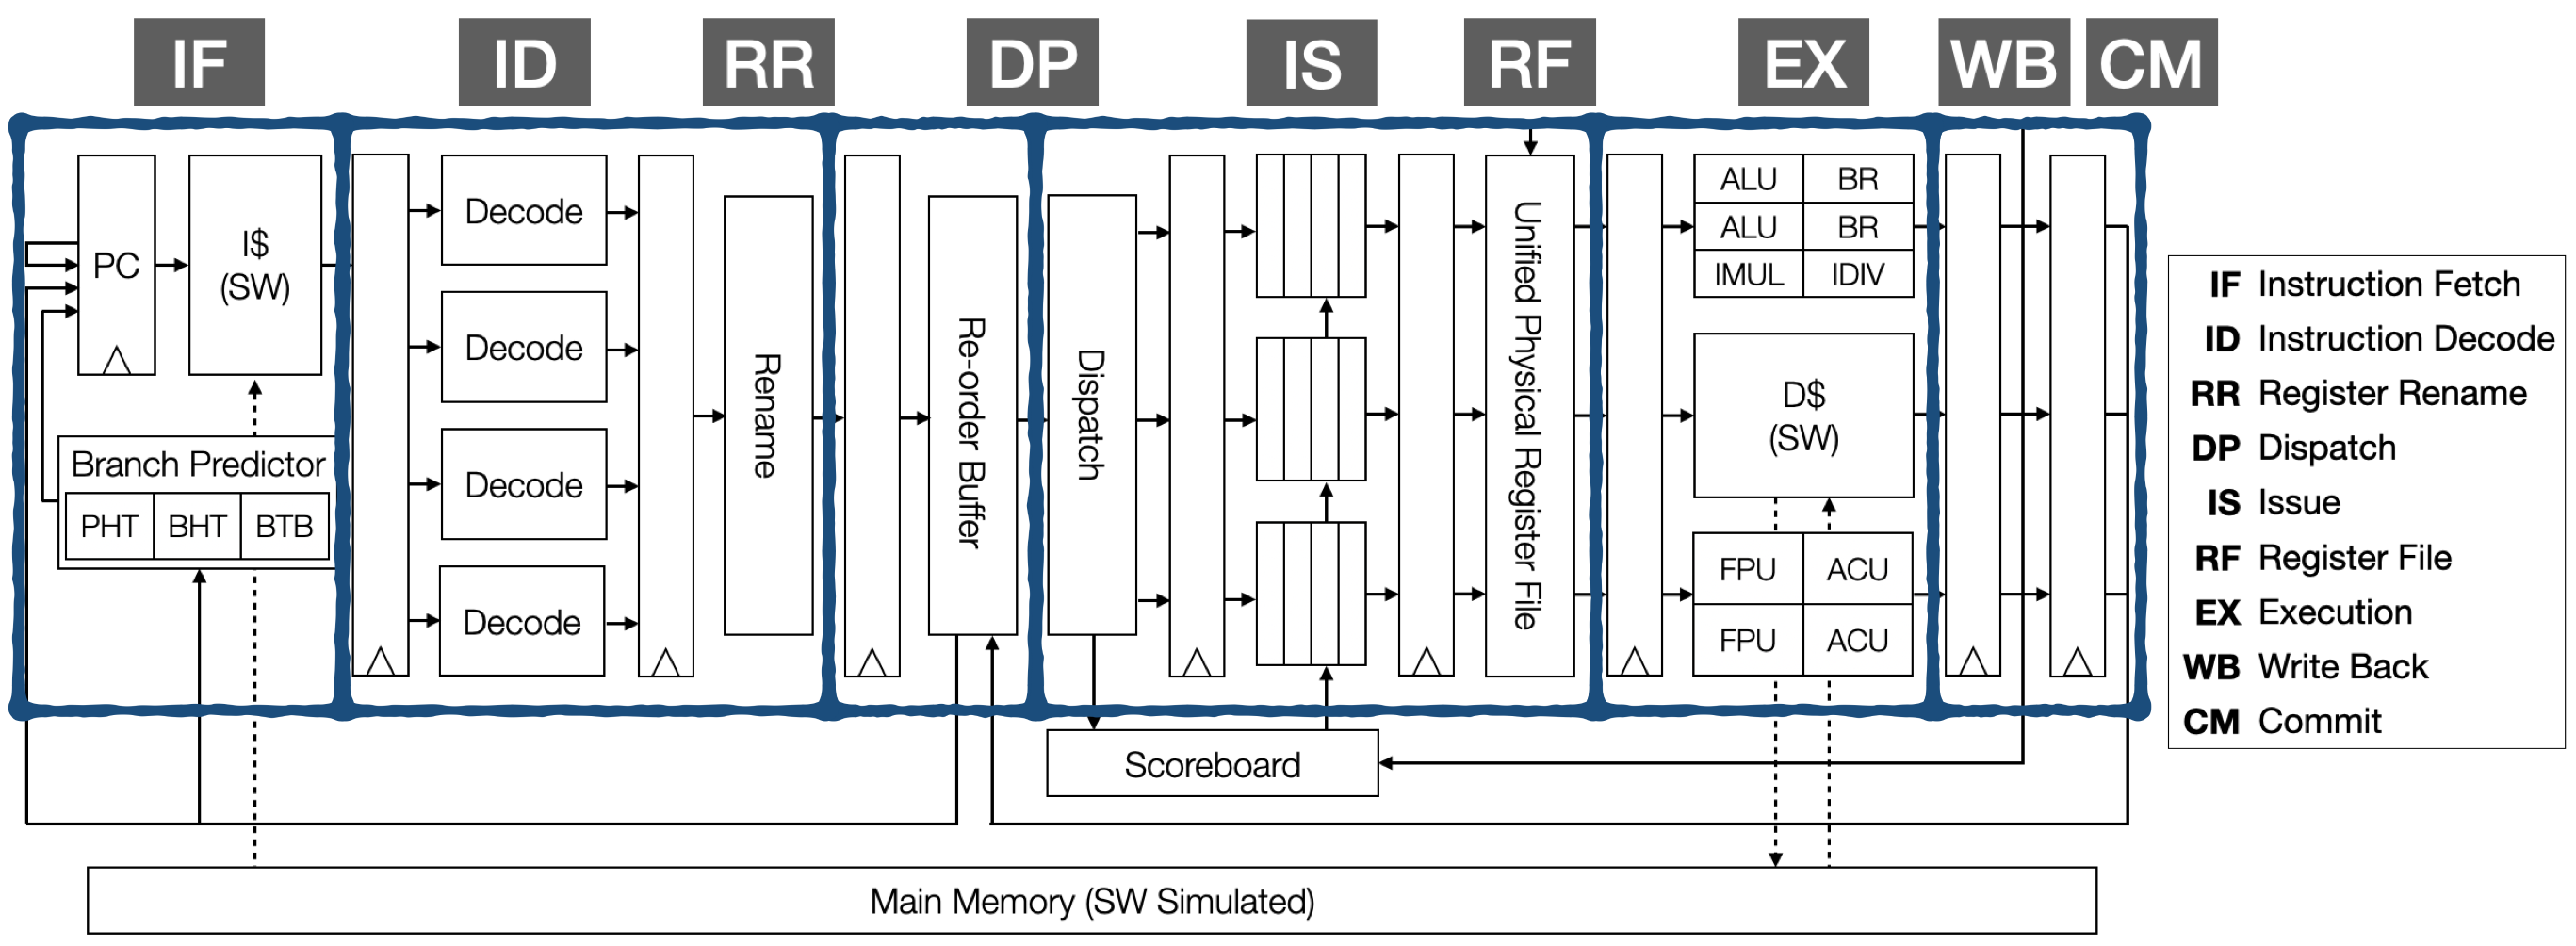
\includegraphics[width=\textwidth]{figure/new_design.png}
    \caption{Optimized RISV-V core design draft}
    \label{fig:opt_core}
\end{figure}

\subsection{Current Solution \& Future Work}
According our discussion in the above Problem section, the possible optimized stage distribution is shown in Fig. \ref{fig:opt_core}. Since it is just an optimization, it won't affect the correctness of the current design. Our current design is still runnable and functionally correct. In the future, we will apply those optimizations and analyze the performance gained from the changes.